\chapter{Il linguaggio IMP}

Per studiare il problema della verifica in programmi imperativi si utilizzerà un piccolo linguaggio di programmazione chiamato \evidence{IMP}\footnote{A volte viene chiamato "while".}. 

\section{Introduzione a IMP}

\dfn{Comandi di IMP}{
  Un programma, in IMP, è un comando con la seguente sintassi:
  
  \begin{center}
    Com $\in$ c, c' ::= \evidence{SKIP} | x := a | c :: c' | \evidence{IF} b \evidence{THEN} c \evidence{ELSE} c' | \evidence{WHILE} b \evidence{DO} c
  \end{center}

}

\nt{La sintassi è simile al Pascal o al C, ma:
\begin{itemize}
  \item [$\Rightarrow$] \evidence{SKIP}: termina l'esecuzione senza effetti collaterali;
  \item [$\Rightarrow$] c :: c' : la composizione (in AGDA è c ; c').
\end{itemize}
}

\cor{Stati di un programma IMP}{
  Un comando, in IMP, è una trasformazione della memoria. 
  Uno \evidence{stato della memoria} (o stato) è una mappatura del tipo \texttt{s : State} con \texttt{State = Varname $\rightarrow$ Val} ossia l'assegnazione di un valore (\texttt{Val}) a ogni variabile (\texttt{Varname}). 
}

\subsection{Le relazioni in IMP}

In IMP esistono due possibili relazioni:

\begin{itemize}
  \item \fancyglitter{Big-step}:  $(\!(c , s)\!)  \Rightarrow t$, dove $(\!(\underline{\hspace{0.4cm}} , \underline{\hspace{0.4cm}})\!) \Rightarrow \underline{\hspace{0.4cm}} \subseteq (\texttt{Com} \times \texttt{State }) \times \texttt{State}$;
  \item \fancyglitter{Small-step}: $(\!( c , s )\!) \rightarrow (\!( c' , t )\!)$, dove $(\!(\underline{\hspace{0.4cm}},\underline{\hspace{0.4cm}})\!) \rightarrow (\!(\underline{\hspace{0.4cm}},\underline{\hspace{0.4cm}})\!) \subseteq (\texttt{Com} \times \texttt{State}) \times (\texttt{Com} \times \texttt{State})$.
\end{itemize}

\thm{Equivalenza di Big-step e Small-step}{
  Big-step e Small-step sono legate dalla seguente relazione:

  $$\forall \text{\textit{c s t . }} (\!( c , s )\!) \Rightarrow t \Longleftrightarrow (\!( c , s )\!) \rightarrow^* (\!( \evidence{SKIP} , t )\!)$$

}

\nt{Dove $\rightarrow^*$ è la relazione meno riflessiva e transitiva che includa $\rightarrow$.}

\subsection{La logica di Floyd-Hoare}

Per compiere la verifica formale di programmi sono necessarie le \fancyglitter{specificazioni}. In questo corso si utilizzano le \fancyglitter{asserzioni}. 

\dfn{Asserzioni}{
  Un'\evidence{asserzione} (\texttt{P : Assn}), dove \texttt{Assn = State $\to$ Set}, è un predicato di stati.
}

\cor{Pre-condizioni e Post-condizioni}{
  Un paio di asserzioni \texttt{P} e \texttt{Q} sono pre-condizioni e post-condizioni di un programma \texttt{c} nella tripla $[\texttt{P}]$ c $[\texttt{Q}]$.
}

\nt{Nei libri di testo le pre-condizioni e le post-condizioni sono segnate come \{\texttt{P}\} c \{\texttt{Q}\}, ma questa notazione \textbf{non} è permessa da AGDA.}

\thm{Correttezza parziale}{
  Una tripla $[\texttt{P}]$ c $[\texttt{Q}]$ è \evidence{valida} ($\models [\texttt{P}]$ c $[\texttt{Q}]$) se per ogni stato \texttt{s} e \texttt{t} se \texttt{P s} e $(\!(c , s)\!)  \Rightarrow t$ allora \texttt{Q t}. 

  In simboli:
      $$\forall \text{\textit{s t . }} P\;\; s \land (\!(c , s)\!)  \Rightarrow t \Longrightarrow Q\;\;t$$

}

\nt{Questa correttezza è solo parziale, perchè le pre-condizioni non sono richieste per dire che il programma c termini partendo da uno stato s}

\section{Espressioni}

In questa sezione si introducono le espressioni \fancyglitter{aritmetiche} (\texttt{Aexp}) e le espressioni \fancyglitter{booleane} (\texttt{Bexpr}). 

\dfn{Variabili}{
  Prendiamo \{$X_0, X_1, \dots$ \} come insieme numerabile di variabili. In AGDA formalizziamo $X_i$ con \texttt{Vn i} ossia la variabile il cui nome ha indice \texttt{i} (\texttt{i} $\in$ \texttt{Index}\footnote{\texttt{Index} è $\bbN$.}).
}

\begin{figure}[h]
  \centering
  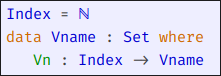
\includegraphics[scale=0.8]{images/IMP/Vname.png}
\end{figure}

\nt{Negli esempi presentati assumeremo X = \texttt{Vn 0}, Y = \texttt{Vn 1} e Z = \texttt{Vn 2}.}

\dfn{Confronto}{
  Per confrontare due variabili definiamo la funzione \texttt{x =Vn y} che compara due nomi e restituisce \texttt{true} se sono gli stessi, \texttt{false} altrimenti. Questa funzione dipende a sua volta da un'altra funzione \texttt{x $=\bbN$ y} per controllare che due $\bbN$ siano uguali.
}

\begin{figure}[h]
  \centering
  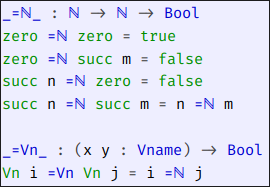
\includegraphics[scale=0.8]{images/IMP/Confronto.png}
\end{figure}


\subsection{Espressioni aritmetiche}

\dfn{Aexp}{
  Si può definire la sintassi delle \evidence{espressioni aritmetiche} (\texttt{Aexp}) con la grammatica:

  \begin{center}
    \texttt{Aexp} $\in$ a, a' ::=  \evidence{N} n | \evidence{V} vn | \evidence{Plus} a a' 
  \end{center}
  Dove n $\in$ \texttt{Nat} e vn $\in$ \texttt{Vname}.
}

\begin{figure}[h]
  \centering
  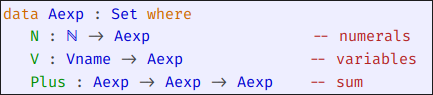
\includegraphics[scale=0.75]{images/IMP/Aexp.png}
\end{figure}

\ex{X + (1 + Y)}{
  aexp0 : \texttt{Aexp}

  aexp0 = Plus (V X) (Plus (N 1) (V Y))
}

\dfn{Stato}{
  Uno \evidence{stato} è una mappatura dai nomi delle variabili ai loro valori:
  \begin{itemize}
    \item [$\Rightarrow$] \texttt{Val} = $\bbN$;
    \item [$\Rightarrow$] \texttt{State} = \texttt{Vname} $\to$ \texttt{Val}. 
  \end{itemize}

  Il significato di stato è un'astrazione della memoria finita di un computer.

}

\nt{Usando questa definizione di stato (che è totale) non si avrà a che fare con funzioni parziali o con il costruttore \texttt{Maybe}.}

\dfn{Aggiornamento}{
L'\evidence{aggiornamento dello stato} è un cambiamento del significato delle singole variabili.

Per formalizzare: l'operatore s [ x ::= v] restituisce lo stato che si comporta come s, ma quando è applicato a X lo trasforma in Y.
}

\begin{figure}[h]
  \centering
  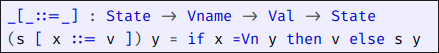
\includegraphics[scale=0.8]{images/IMP/Update.png}
\end{figure}

\ex{Stati}{
\begin{center}
  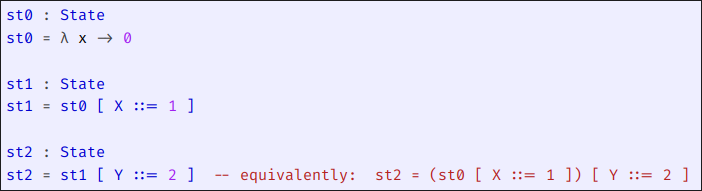
\includegraphics[scale=0.6]{images/IMP/Stati.png}
\end{center}
}

\dfn{Aval}{
  La funzione \texttt{aval} è un'interpretazione di \texttt{Aexpr} utilizzando gli stati.
}

\begin{figure}[h]
  \centering
  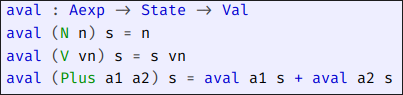
\includegraphics[scale=0.6]{images/IMP/Aval.png}
\end{figure}

\begin{itemize}
  \item Il caso \fancyglitter{N} n non dipende dallo stato, ma restituisce solo n;
  \item Il caso \fancyglitter{V} vn restituisce il valore dello stato s quando applicato a vn\footnote{Ovvero il suo valore salvato in memoria, come nei registri in Assembly.};
  \item Il caso \fancyglitter{Plus} a1 a2 restituisce la somma aritmetica della valutazione ricorsiva su a1 e a2. 
\end{itemize}

\subsection{Sostituzione}

\dfn{Sostituzione}{
  La \evidence{sostituzione} consiste nel rimpiazzare ogni occorrenza di una varibile x in un'espressione a con un espressione a'.
}

\begin{figure}[h]
  \centering
  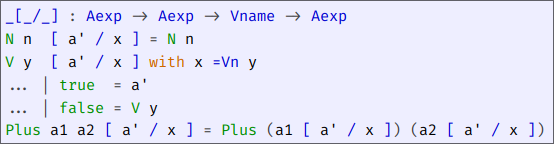
\includegraphics[scale=0.7]{images/IMP/Sostituzione.png}
\end{figure}

\ex{(X + (1 + Y)) [ (Z + 3) / X ]}{
  aexp1 : \texttt{Aexp}

  aexp1 = aexp0 [ Plus (V Z) (N 3) / X ]
}

\mlenma{Sostituzione}{
  Sostituendo x con a' in a e valutando il risultato si ottiene lo stesso stato s che si otterrebbe valutando x nello stato s [ x ::= (aval a' s) ], ossia lo stato in cui il valore di x è stato aggiornato con il valore di a'.
}

\begin{figure}[h]
  \centering
  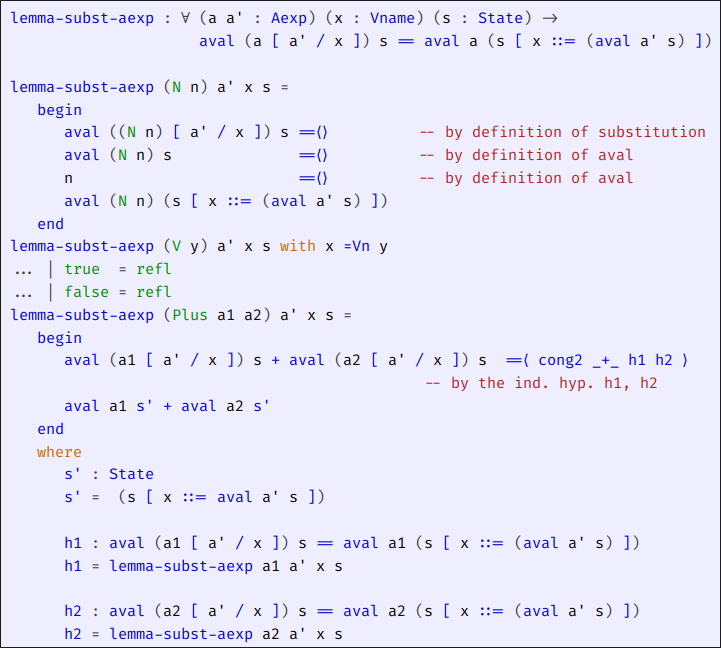
\includegraphics[scale=0.5]{images/IMP/Lsub.png}
\end{figure}

\paragraph{Step della prova:}

\begin{enumerate}
  \item Per prima cosa si fa induzione su a;
  \item Il caso a = \fancyglitter{N} n: banale, perchè non può comparire la x essendo n un numerale;
  \item Il caso a = \fancyglitter{V} y: viene risolto mediante l'utilizzo del costrutto \texttt{with};
  \item Il caso a = \fancyglitter{Plus} a1 a2: si utilizzano le ipotesi induttive perchè ne è la diretta conseguenza.
\end{enumerate}

\subsection{Espressioni booleane}
\dfn{Bexp}{
  Si può definire la sintassi delle \evidence{espressioni aritmetiche} (\texttt{Aexp}) con la grammatica:
  
  \begin{center}
  \texttt{Bexp} $\in$ b, b' ::= B bc | \evidence{Less} a a' | \evidence{Not} b | \evidence{And} b b'
  \end{center}
  Dove bc $\in$ \texttt{Bool} e a, a' $\in$ \texttt{Aexp}.
}

\begin{figure}[h]
  \centering
  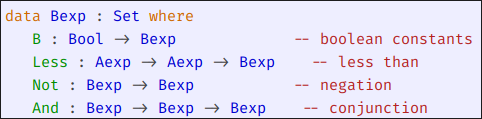
\includegraphics[scale=0.75]{images/IMP/Bexp.png}
\end{figure}

\ex{Alcuni esempi}{
  bexp1 : \texttt{Bexp}

bexp1 = Not (Less (V X) (N 1))      

\subsubsection{}

bexp2 : \texttt{Bexp}

bexp2 = And bexp1 (Less (N 0) (V Y)) 
}

\dfn{Confronto}{
  La valutazione delle espessioni booleane dipende dalla valutazione delle espressioni aritmetiche e quindi, indirettamente, dallo stato.
}


\begin{figure}[h]
  \centering
  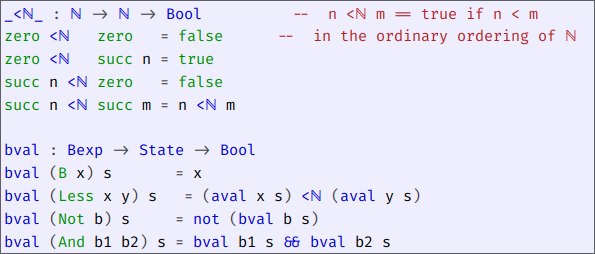
\includegraphics[scale=0.75]{images/IMP/Confronto1.png}
\end{figure}

\pagebreak

\section{Semantica Big-step}

Tra le due possibili semantiche operazionali la Big-step è un approccio astratto basato sulla nozione di \fancyglitter{convergenza}. 

\subsection{Comandi}

\dfn{Comandi}{
  La sintassi dei \evidence{comandi} si basa sulla grammatica:
  \begin{center}
    \texttt{Com} $\in$ c, c' ::= \evidence{SKIP} | x := a | c :: c' | \evidence{IF} b \evidence{THEN} c \evidence{ELSE} c' | \evidence{WHILE} b \evidence{DO} c
  \end{center}

  Dove x $\in$ \texttt{Vname}, a $\in$ \texttt{Aexp} e b $\in$ \texttt{Bexp}.

}

\begin{figure}[h]
  \centering
  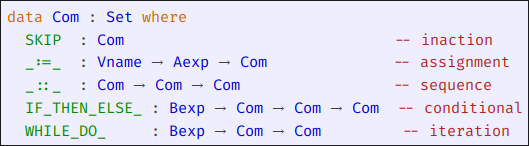
\includegraphics[scale=0.9]{images/IMP/Comandi.png}
\end{figure}

\subsection{Convergenza}

\dfn{Predicato di convergenza}{
  La relazione  $(\!(c , s)\!)  \Rightarrow t$ significa che l'esecuzione di c, quando inizia in s, termina in t. 
}

\nt{
  Questo in generale può richiedere una serie di step che sono racchiusi in un unico Big-step.
}

\cor{Configurazioni}{
  Chiamiamo \evidence{configurazioni} ogni coppia  $(\!(c , s)\!)$ comando-stato. 
}

\begin{figure}[h]
  \centering
  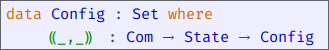
\includegraphics[scale=1]{images/IMP/Configurazioni.png}
\end{figure}

\pagebreak

\dfn{Relazione}{
  Si definisce la relazione $\Rightarrow$ tra \texttt{Config} e \texttt{State} per creare un sistema formale. 
}


\begin{figure}[h]
  \centering
  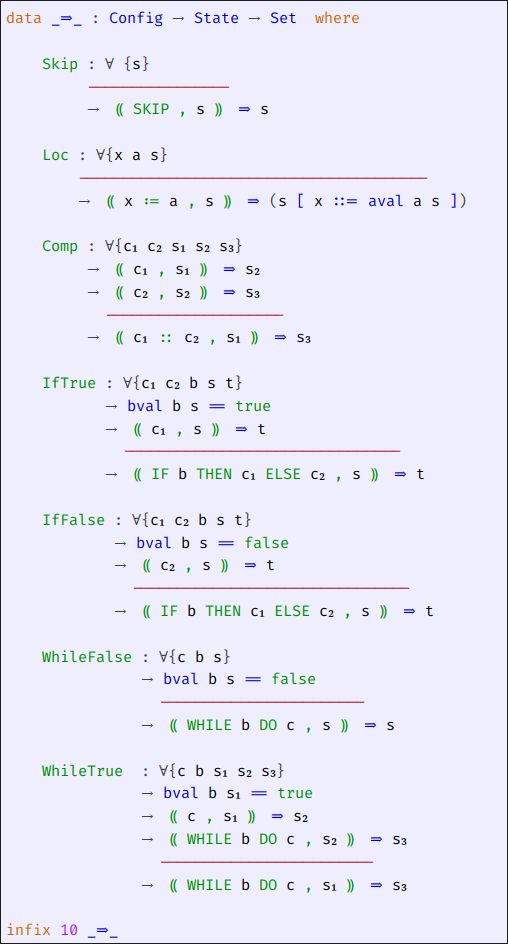
\includegraphics[scale=0.55]{images/IMP/Rel.png}
\end{figure}

\pagebreak

\subsection{Proprietà della convergenza}

\thm{Non trivialità}{
  Esiste almeno un comando che non produce nessuno stato finale come risultato della sua esecuzione.
}

\nt{L'esempio più naturale è \fancyglitter{WHILE} B true \fancyglitter{DO} c.}

\begin{figure}[h]
  \centering
  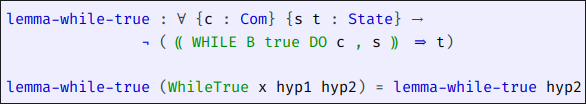
\includegraphics[scale=0.55]{images/IMP/Wtrue.png}
\end{figure}

\begin{itemize}
  \item La prova di questo lemma è per contraddizione;
  \item hyp1 = $(\!(c , s)\!) \Rightarrow s_2$;
  \item hyp2 = $(\!(\text{WHILE B true DO c}, s_2)\!) \Rightarrow t$.
\end{itemize}

\nt{Non è una Reductio Ad Absurdum, ma una semplice prova per contraddizione.}

\thm{Determinismo}{
  Ogni volta che  $(\!(c , s)\!)  \Rightarrow t$ è derivabile per qualche  $(\!(c , s)\!)  \in \text{\texttt{Config}}$ e $t \in$ \texttt{State}, lo stato $t$ è unico.
}

\nt{Per provare questo teorema abbiamo bisogno di due lemmi.}

\mlenma{Una cosa o è vera o è falsa}{

  \begin{center}
    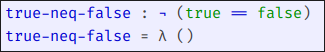
\includegraphics[scale=0.75]{images/IMP/VF.png}
  \end{center}
}

\mlenma{Il vero è diverso dal falso}{

  \begin{center}
    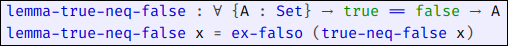
\includegraphics[scale=0.75]{images/IMP/LVF.png}
  \end{center}
}

\pagebreak

  \begin{center}
    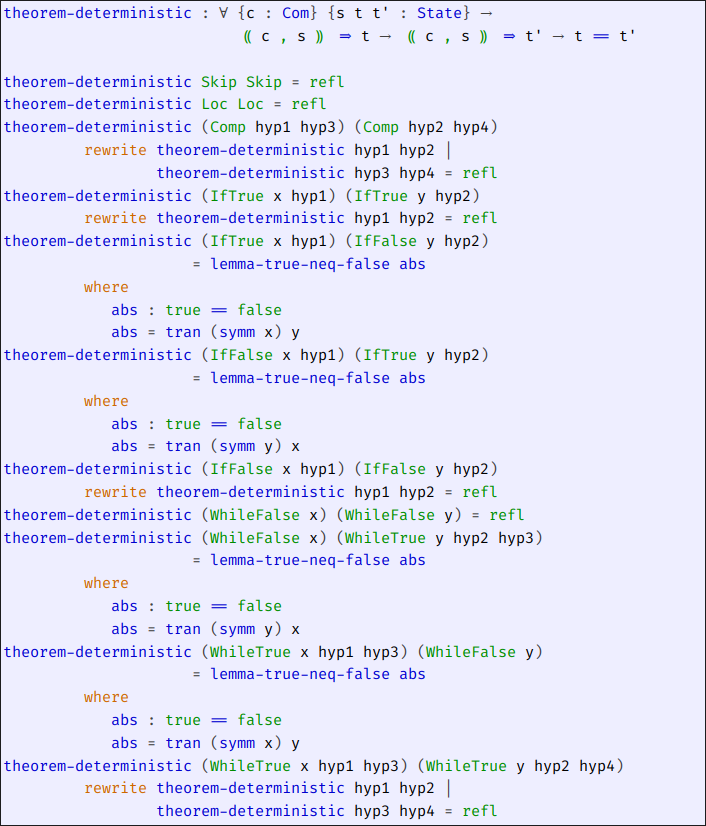
\includegraphics[scale=0.65]{images/IMP/Det.png}
  \end{center}

  \nt{La prova consiste semplicemente in due induzioni simultanee sulle ipotesi $(\!(c , s)\!)  \Rightarrow t$ e $(\!(c , s)\!)  \Rightarrow t'$, usando la tattica \evidence{rewrite}. I due lemmi dimostrati in precedenza sono utili per gestire i casi impossibili riducendoli all'assurdo (ex-falso).}

\subsection{Equivalenza}

\dfn{Equivalenza}{
  Due comandi c, c' $\in$ \texttt{Com} sono equivalenti per ogni s $\in$ \texttt{State} delle computazioni $(\!(c , s)\!)$ e  $(\!(c , s)\!)$ non convergono o $(\!(c , s)\!)  \Rightarrow t$ e  $(\!(c' , s)\!)  \Rightarrow t$  per ogni t $\in$ \texttt{State}. 
}


\begin{center}
 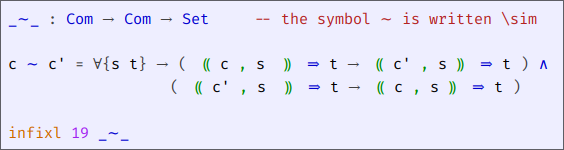
\includegraphics[scale=0.65]{images/IMP/Equivalenza.png}
\end{center}

\nt{L'equivalenza tra i comandi è utilizzata per ottimizzazioni.}

\ex{IF}{

In questo esempio l'IF può essere rimosso perchè sia che la condizione sia vera sia che sia falsa eseguirà sempre lo stesso comando.

  \begin{center}
    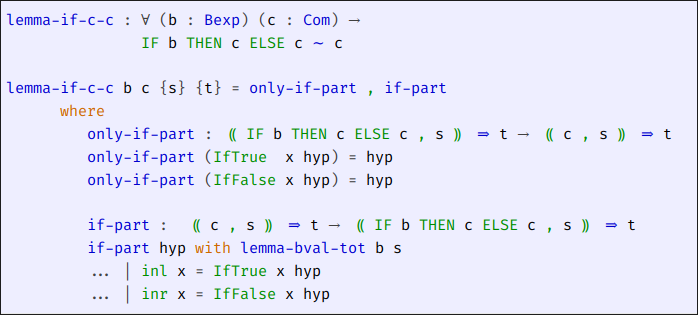
\includegraphics[scale=0.65]{images/IMP/If.png}
  \end{center}

  lemma-bval-tot è un lemma per cui la valutazione di un espressione booleana restituisce o true o false.

}

\pagebreak

\section{Semantica Small-step}

Un approccio alternativo alle semantiche operazionali è quello di descrivere la computazione come l'esecuzione di una serie di step.

\subsection{Riduzione in un passo}

\dfn{Relazione di riduzione in un passo}{
  La relazione $(\!( c , s )\!) \longrightarrow (\!( c' , s' )\!)$ modella l'esecuzione del comando "più a sinistra" in $c$ iniziando da $s$, producendo la nuova configurazione $(\!( c' , s' )\!)$
dove $c'$ (\evidence{continuazione}) è ciò che resta da eseguire di $c$ e $s'$ è il nuovo stato 
prodotto. La relazione $\longrightarrow$ è chiamata \evidence{riduzione in un passo}.

}

\begin{center}
  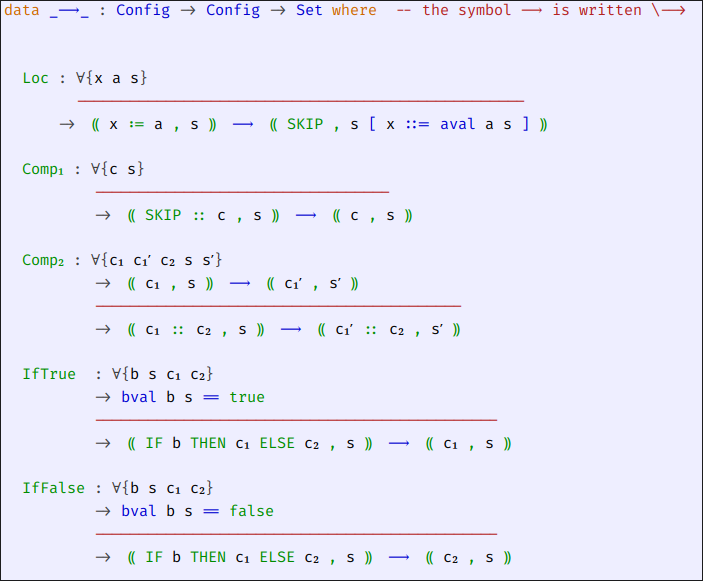
\includegraphics[scale = 0.5]{images/IMP/R1.png}
  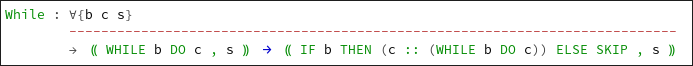
\includegraphics[scale = 0.51]{images/IMP/R2.png}
\end{center}

\begin{itemize}
  \item \fancyglitter{SKIP} è il comando terminale, quindi non riduce a niente e tutti i comandi che lo raggiungono sono terminati;
  \item \fancyglitter{Comp$_1$} indica che il primo comando è terminato e quindi l'esecuzione continua con il prossimo;
  \item \fancyglitter{Comp$_2$} indica che il primo comando si può ridurre a un comando diverso da SKIP;
  \item \fancyglitter{IfTrue} e \fancyglitter{IfFalse} sono banali, perché IfTrue esegue il ramo THEN e IfFalse esegue il ramo ELSE;
  \item \fancyglitter{While} si comporta come in un generico linguaggio di programmazione in cui controlla (mediante If) a ogni iterazione. Se è true continua, mentre se è false diventa SKIP (termina).
\end{itemize}

\pagebreak

\subsection{Chiusure}

\dfn{Riduzione in più passi}{
  La \evidence{riduzione in più passi} (o riduzione) è la chiusura transitiva e riflessiva della riduzione in un passo.
}


\begin{center}
  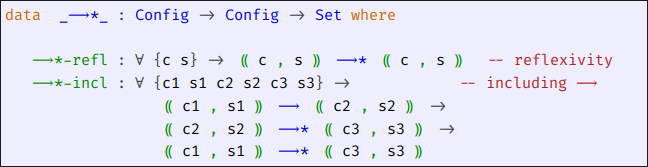
\includegraphics[scale = 0.55]{images/IMP/C1.png}
\end{center}

\begin{itemize}
  \item La regola \fancyglitter{$\longrightarrow$*-refl} postula la riflessività;
  \item La regola \fancyglitter{$\longrightarrow$*-incl} concatena la riduzione in un passo alla riduzione in più passi\footnote{Ricorda il cons nelle liste.}.
\end{itemize}

\nt{Da queste si deriva la regola di transitività.}

\begin{center}
  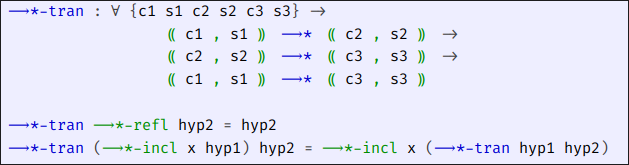
\includegraphics[scale = 0.55]{images/IMP/C2.png}
\end{center}

\paragraph{In AGDA andremo a utilizzare le seguenti macro.}

\begin{center}
  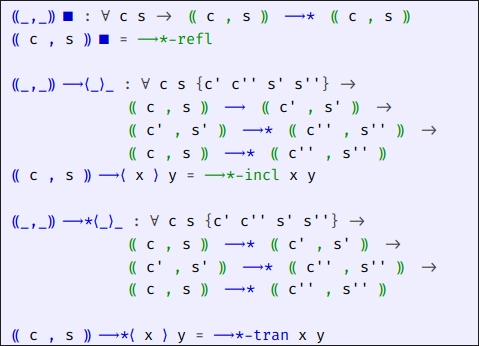
\includegraphics[scale = 0.75]{images/IMP/Macro.png}
\end{center}

\pagebreak

\section{Relazione tra semantica Big-step e semantica Small-step}



